\subsubsection{Aufbau}
In der physischen Zelle wird durch zwei Rampen (Lagerplätze) und einen Volksbot (AGV) ein kleines Umschlagslager dargestellt. Zudem können über ein \textsc{Mica}z-Modul, das als Gateway fungiert, Agenten-Nachrichten und damit etwa Pakete oder Aufträge in das System eingespeist werden.

\autoref{fig:physischeZelle} zeigt den Beispielaufbau. Die beiden Rampen A und B sind über den Volksbot in der Lage, Pakete auszutauschen. Initialisiert werden sowohl Pakete als auch entsprechende Aufträge für diese Pakete über das \textsc{Mica}z-Gateway unten links.

\begin{figure}[h!]
	\centering
		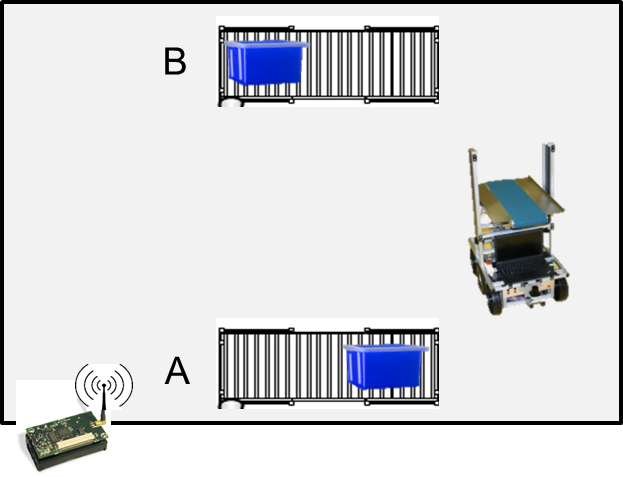
\includegraphics[width=0.5\textwidth]{physischeZelle.png}
	\caption{Aufbau der physischen Zelle}
	\label{fig:physischeZelle}
\end{figure}

Auf allen Modulen (Rampen und Volksbots) sind \textsc{Mica}z-Module angebracht, die sich um die Betriebslogik kümmern und etwa den Volksbots ihre nächsten Ziele zuweisen. Die \textsc{Mica}z-Module kommunizieren dabei untereinander drahtlos auf Agentenbasis (siehe \autoref{sec:FlowAgents}). Die Module auf den Volksbots kommunizieren außerdem mit den auf den Volksbots angebrachten Laptops über eine UART-Schnittstelle. Das entsprechende Protokoll ist in den Tabellen \ref{tab:UART_FD} und \ref{tab:UART_DF} zu sehen. Jede Nachricht hat dabei genau fünf Byte, ein Byte Opcode und bis zu vier Byte Daten. Benötigt ein Befehl weniger Daten, werden die restlichen Bytes mit Nullen aufgefüllt.

Ausgehende Nachrichten auf Seiten der \textsc{Mica}z-Module werden dabei direkt über das UART-Interface verschickt, während eingehende Nachrichten vom CommunicationInterface aufbereitet und dem jeweiligen Zielagent als Agentennachrichten bereitgestellt werden. So kann die asynchrone UART-Nachricht vom Agenten bei seinem nächsten Aufruf abgerufen und verarbeitet werden.

\begin{table}[h!]
\centering
\begin{tabular}{| l | l | l | l |}
  \hline
  Nachricht & Opcode & Parameter & Agent (\textsc{Mica}z)\\
  \hline
  Kostenanfrage & 0x10 & Start-ID + Ziel-ID & Routing-Agent\\
  Hole Paket ab & 0x02 & Rampen-ID & Plattform-Agent\\
  Transportiere Paket & 0x01 & Rampen-ID & Plattform-Agent \\
  \hline
\end{tabular}
\caption{UART-Kommunikation von \textsc{Mica}z-Modul zu Volksbot}
\label{tab:UART_FD}
\end{table}

\begin{table}[h!]
\centering
\begin{tabular}{| l | l | l | l |}
  \hline
  Nachricht & Opcode & Parameter & Zielagent (\textsc{Mica}z) \\
  \hline
  Antwort auf Kostenanfrage & 0x11 & Start-ID + Kosten & Routing-Agent \\
  Rampe mit Paket erreicht & 0x50 & Rampen-ID & Plattform-Agent\\
  Rampe ohne Paket erreicht & 0x55 & Rampen-ID & Plattform-Agent\\
  \hline
\end{tabular}
\caption{UART-Kommunikation von Volksbot zu \textsc{Mica}z-Modul}
\label{tab:UART_DF}
\end{table}